\begin{center}
\footnotesize (El la \emph{Revue Bourguignonne,} publikigata de la Universitato de
Dijon).
\end{center}

   Multaj homoj en \^ciu lando laboras nun por la propagando de la bela
lingvo internacia. La junaj fra\u uloj a\u u fra\u ulinoj sin \^goje
amuzas, skribante, legante, parolante pri \^ciuj objektoj de la
mondo, precipe pri la plej konformaj al sia feli\^ca a\^go. Ili tiel
pruvas, pli kaj pli, la mirindan kapablon de Esperanto esprimi tute
la delikata\^{\j}ojn de la spirito kaj de la koro. La maljunaj, miaj
egala\^guloj, aliflanke, povas pruvi, ke tiu kapablo ne estas malpli
mirinda por skribi, legi, paroli pri \^ciuj objektoj sciencaj.

   Hodia\u u mi do volas, malgra\u u malforti\^go pro laceco kaj klopodoj, en
la kelkaj sekvontaj linioj, doni rapide la priskribon kaj teorion de
la sunhorlo\^go, ku\^santa en la fundo de la \^carma Parko de Dijon,
sur la bordo de la beleta rivero nomata {\sl Ouche}.

\begin{center}
\begin{tikzpicture}[every node/.style={font=\footnotesize\sansfont,inner sep=0pt}]
%
%
\draw (0,-3.5) -- (0,3.5); % NS axis
\draw (-4.5,0) -- (4.5,0); % EO axis
% main ellipse
\node[draw,ellipse,minimum height=0.5\textwidth,minimum width=0.75\textwidth] (ell) at (0,0) {};
%
% points around the ellipse, with the number, direction, and axis labels
%
\node[draw,circle,fill=black,
	minimum size=4pt,
	label={[label distance=3pt]45:6},
	label={[label distance=3pt]315:x},
	label={[label distance=3pt]225:E}] (6e) at (ell.0) {};
\node[draw,circle,fill=black,minimum size=4pt,label={[label distance=3pt]45:5}] (5e) at (ell.12.75) {};
\node[draw,circle,fill=black,minimum size=4pt,label={[label distance=3pt]45:4}] (4e) at (ell.25.7) {};
\node[draw,circle,fill=black,minimum size=4pt,
	label={[label distance=3pt]45:3},
	label={[label distance=0.5cm]3:M(x,y)}] (3e) at (ell.39.5) {};
\node[draw,circle,fill=black,minimum size=4pt,label={[label distance=3pt]45:2}] (2e) at (ell.55) {};
\node[draw,circle,fill=black,minimum size=4pt,label={[label distance=3pt]45:1}] (1e) at (ell.72.7) {};
\node[draw,circle,fill=black,
	minimum size=4pt,
	label={[label distance=3pt]135:12},
	label={[label distance=3pt]45:y},
	label={[label distance=3pt]315:N}] (12n) at (ell.90) {};
\node[draw,circle,fill=black,minimum size=4pt,label={[label distance=3pt]135:11}] (11o) at (ell.107.3) {};
\node[draw,circle,fill=black,minimum size=4pt,label={[label distance=3pt]135:10}] (10o) at (ell.125) {};
\node[draw,circle,fill=black,minimum size=4pt,label={[label distance=3pt]135:9}] (9o) at (ell.140.5) {};
\node[draw,circle,fill=black,minimum size=4pt,label={[label distance=3pt]135:8}] (8o) at (ell.154.3) {};
\node[draw,circle,fill=black,minimum size=4pt,label={[label distance=3pt]135:7}] (7o) at (ell.167.25) {};
\node[draw,circle,fill=black,
	minimum size=4pt,
	label={[label distance=3pt]135:6},
	label={[label distance=3pt]315:O}] (6o) at (ell.180) {};
\node[draw,circle,fill=black,minimum size=4pt,label={[label distance=3pt]225:5}] (5o) at (ell.192.5) {};
\node[draw,circle,fill=black,minimum size=4pt,label={[label distance=3pt]225:4}] (4o) at (ell.205.7) {};
\node[draw,circle,fill=black,minimum size=4pt,label={[label distance=3pt]225:3}] (3o) at (ell.219.5) {};
\node[draw,circle,fill=black,minimum size=4pt,label={[label distance=3pt]225:2}] (2o) at (ell.235) {};
\node[draw,circle,fill=black,minimum size=4pt,label={[label distance=3pt]225:1}] (1o) at (ell.252.7) {};
\node[draw,circle,fill=black,
	minimum size=4pt,
	label={[label distance=3pt]45:S},
	label={[label distance=3pt]315:12}] (12s) at (ell.270) {};
\node[draw,circle,fill=black,minimum size=4pt,label={[label distance=3pt]315:11}] (11e) at (ell.287.3) {};
\node[draw,circle,fill=black,minimum size=4pt,label={[label distance=3pt]315:10}] (10e) at (ell.305) {};
\node[draw,circle,fill=black,minimum size=4pt,label={[label distance=3pt]315:9}] (9e) at (ell.320.5) {};
\node[draw,circle,fill=black,minimum size=4pt,label={[label distance=3pt]315:8}] (8e) at (ell.334.3) {};
\node[draw,circle,fill=black,minimum size=4pt,label={[label distance=3pt]315:7}] (7e) at (ell.347.25) {};
%
% lettered rectangles
%
\node[draw,rectangle,minimum height=5mm,minimum width=10mm] (topC) at (0,1.5) {\normalsize c};
\node[draw,rectangle,minimum height=5mm,minimum width=5mm] (lgL) at (-0.25,1) {\normalsize l};
\node[draw,rectangle,minimum height=5mm,minimum width=5mm] (lgG) at (0.25,1) {\normalsize g};
\node[draw,rectangle,minimum height=5mm,minimum width=5mm] (vtV) at (-0.25,0.5) {\normalsize v};
\node[draw,rectangle,minimum height=5mm,minimum width=5mm] (vtT) at (0.25,0.5) {\normalsize t};
\node[draw,rectangle,minimum height=5mm,minimum width=5mm] (laL) at (-0.25,0) {\normalsize l};
\node[draw,rectangle,minimum height=5mm,minimum width=5mm] (laA) at (0.25,0) {\normalsize a};
\node[draw,rectangle,minimum height=5mm,minimum width=5mm] (spS) at (-0.25,-0.5) {\normalsize s};
\node[draw,rectangle,minimum height=5mm,minimum width=5mm] (spP) at (0.25,-0.5) {\normalsize p};
\node[draw,rectangle,minimum height=5mm,minimum width=5mm] (aa1) at (-0.25,-1) {\normalsize a};
\node[draw,rectangle,minimum height=5mm,minimum width=5mm] (aa2) at (0.25,-1) {\normalsize a};
\node[draw,rectangle,minimum height=5mm,minimum width=10mm] (botC) at (0,-1.5) {\normalsize c};
%
%
\end{tikzpicture}
\end{center}


   Sur la tero horizonta estas desegnitaj la du linioj NS (nordo-sudo)
kaj EO (oriento-okcidento) sin kruci\^gantaj rektangule en I. Du
dekduoj da markoj \^stonaj estas plantitaj, \^cirka\u u I, la\u u
la fig.\,1. Sur \^stono la\u ulonge de la linio SN estas markitaj
punktoj kun la signoj de la zodiako, de {\sl kankro al kapro}, sur
unu flanko de SN, kaj de {\sl kapro al kankro} sur la alia flanko.
\^Ciu promenanto tra la Parko, kiu volas scii la horon, iru stari
rekte sur la punkto zodiaka respondanta al la tago de lia promenado
kaj li vidos sian ombron direktatan al la punkto \^stona markita per
la horo ser\^cata.

   Oni vidas ke en tiu \^ci horlo\^go:

1\textsuperscript{o} La ombro\^{\j}etilo estas movebla, sed \^ciam vertikala,
kaj staranta sur NS, en iu punkto A, kies interspaco $\delta$ al I
estas funkcio nur de la deklini\^go D de la suno;

2\textsuperscript{o} La koordinatoj $x, y$ de \^ciu marko \^stona M estas funkcioj nur de
la horo $h$, videble skribita sur M.

   Komparante la sunhorlo\^gon kun bona po\^shorlo\^go, oni certi\^gos pri
la \^gusteco de la unua.

   Mi scias nek la epokon nek la uzitan manieron de la konstruo de
tiu \^ci sunhorlo\^go; kaj mi ne konas, alian ekzempleron de tia en
iaj urboj a\u u libroj. Sed tion \^ci nia eminenta kolego Charles
Méray povus, sendube, al ni sciigi; mi do petas lin ke li volu
skribi la historion de tiu malofta horlo\^go en Esperanto, lingvo,
en kiu li estas tiel majstro kiel en matematiko.

   Atendante tiun historion, oni vidos facile la eblon konstrui \^guste
tian sunhorlo\^gon, se oni ser\^cos la formulojn liverantajn $x, y$
kaj $\delta$.

   Oni nomu:
   
{\newlength{\tempindent}
\setlength{\tempindent}{\parindent}
\setlength{\parindent}{0pt}   
\vspace{1ex}
\hspace*{\tempindent}$\delta$ la kolatitudon de la loko.\\
\hspace*{\tempindent}$a$ la azimuton de la suno.\\
\hspace*{\tempindent}D \^gian deklini\^gon.\\
\hspace*{\tempindent}$h$ \^gian angulon horan a\u u la horon veran.
\vspace{1ex}
}

   Oni scias, ke la triangulo formita, sur la sfero \^ciela, per la polo,
la zenito kaj la suno donas:

\begin{equation}
\text{kot } a  = \frac{\text{kos } \varphi \text{ kos } h - \text{sin } \varphi \text{ tg D} }{\text{sin } h}
\tag{1}
\end{equation}

\begin{center}
\begin{tikzpicture}[every node/.style={font=\normalsize\sansfont,inner sep=0pt}]
%
% axis labels and axes
\node[label={[label distance=3pt]0:y}] (ylabel) at (0,5) {}; 
\node[label={[label distance=3pt]270:x}] (xlabel) at (5.5,0) {};
\draw (0,-1.5) -- (ylabel); % y axis
\draw (-1.5,0) -- (xlabel); % x axis
% A-M line 
\node[label={[label distance=3pt]180:A}] (A) at (0,2) {};
\node[label={[label distance=3pt]0:M(x,y)}] (M) at (4,5) {};
% we give the coordinates for A instead of the node itself so that the line meets the axis
\draw (0,2) -- (M);
% line down from M to x axis
\draw[dashed] (4,0) -- (M);
% line below A-M, parallel to it
\node[] (Aprime) at (-1.2,-.9) {};
\node[] (Mprime) at (4,3) {};
\draw (Aprime) -- (Mprime);
% delta label at origin
\node[label={[label distance=3pt]135:\large$\delta$}] (delta) at (0,0) {};
% arc
\draw[-{Latex[scale=1.25]},dashed] (0,-1) arc (270:216.9:1);
\node[label=225:a] (alabel) at (-0.5,-1) {}; 
%
%
\end{tikzpicture}
\end{center}

   Por ke la ombro de ombro\^{\j}etilo, vertikale metila en A, pasu tra la
punkto M $(x, y)$ respondanta al $h$, estas necesa la rilato

\begin{equation}
\delta  =  y - x \text{ kot } a
\tag{2}
\end{equation}

   evidenta per la fig. 2: Sed devas dependi $x, y$ nur de $h$, kaj $\delta$ nur
de D; oni do havas

\[\frac{\text{d}\varphi}{\text{d}h} = 0\]

a\u u

\begin{equation}
\frac{dy}{dh} =
x \frac{\text{d kot } a}{\text{d}h} + \frac{dx}{dh} \text{ kot } a
\tag{3}
\end{equation}

   Sekve, metinte anstata\u u $kot~a$ kaj {\Large $\frac{d\text{ kot }a}{dh}$} iliajn valorojn eltiritajn el la formulo (1), oni havas

\begin{small}
\begin{equation}
\frac{dy}{dh} = \frac{\text{sin }\varphi}{\text{sin }h} \text{ tg D } \left( x \text{ kot } h - \frac{dx}{dh} \right) - \frac{\text{kos }\varphi}{\text{sin}^2 h} \left( x - \frac{dx}{dh}\text{ sin }h\text{ kos }h \right)
\tag{4}
\end{equation}
\end{small}

   Por ke $y$ dependu nur de $h$, estas necese nuligi la koeficienton de $tg$ D, a\u u skribi

\[\frac{x}{d} = \text{kot }h \cdot dh\]

de kie

\[x = \text{C sin }h\]

C estante konstanto arbitra. Sekve (4) donas

\[\frac{dy}{dh} = \text{C}\frac{\text{kos }\varphi}{\text{sin }h} \left(-1 + \text{kos}^2 h \right) =  \text{C kos }\varphi\text{ sin } h,\]

de kie

\[y = \text{C kos }\varphi\text{ kos }h + \text{C}';\]

tie \^ci C$'$ estas alia konstanto arbitra. Fine (2) liveros:

\begin{gather*}
\delta = \text{C kos }\varphi\text{ kos }h + \text{C}' - \text{C}(\text{kos }\varphi\text{ kos }h - \text{sin }\varphi\text{ tg D})\\
         = \text{C sin }\varphi\text{ tg D} + \text{C}'.
\end{gather*}

Resume, oni vidas ke:

1\textsuperscript{o} La \^stonaj markoj estas trovitaj per

\begin{center}
$x = \text{C sin }h$,\hspace{0.5cm}$y = \text{C kos }\varphi\text{ kos }h + \text{C}'$
\end{center}

kaj metitaj sur la elipso

\[\frac{x^2}{\text{C}^2} + \frac{(y - \text{C}')^2}{\text{C}^2\text{ kos}^2 \varphi} = 1.\]

2\textsuperscript{o} La zodiakaj punktoj estas trovitaj per

\[\delta = \text{C sin }\varphi \text{ tg D } + \text{C}'.\]

   La konstruinto de la horlo\^go Dijona elektis $\text{C}'=0$ pro simpleco, kaj
C de longeco agrabla rilate al la lar\^geco de la vojo kondukanta
al tiu horlo\^go tiel stranga kaj interesa.

   Nuligante C$'$, oni havas:

\begin{gather*}
x = \text{C sin }h \hspace{0.5cm};\hspace{0.5cm} y = \text{C kos }h\text{ kos }\varphi \tag{5}\\
\delta = \text{C tg D sin }\varphi. \tag{6}
\end{gather*}

   La formuloj (5) montras, videble, ke M estas la projekcio horizonta
de la punkto $m$, kiu respondas al la horo $h$ sur la rondo
tagnoktegaliga, farita per la radio C priskribita.

   La formulo (6) montras, same videble, ke $\delta$ estas la projekcio
horizonta de la longo C $tg$ D, metita sur la polusojlinio de
la centro I de la sfero \^ciela al la nordo a\u u la sudo, la\u u
tio ke D estas norda a\u u suda.

   Se do oni konsideras sunhorlo\^gon tagnoktegaligan, kies ombro\^{\j}etilo
estas de longeco C $tg$ D, \^san\^ganta la\u utage, oni povas
diri:

   La sunhorlo\^go Dijona estas la projekcio horizonta de la sunhorlo\^go
tagnoktegaliga.

   Tiu tre simpla rezultato estas videbla geometrie, en la sekvanta
maniero:

\begin{center}
\resizebox{0.45\textwidth}{!}{%
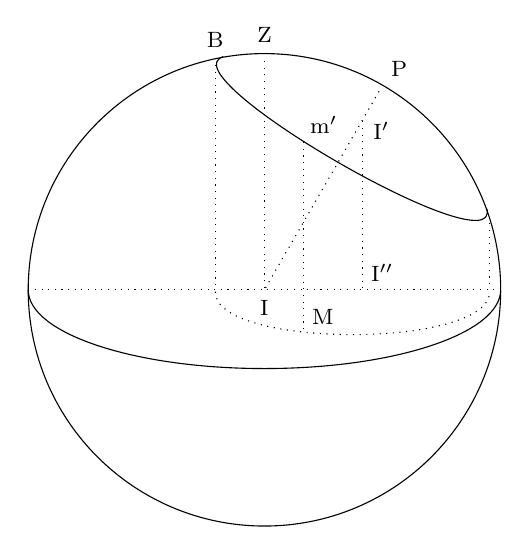
\begin{tikzpicture}[every node/.style={font=\footnotesize\sansfont,inner sep=0pt}]
%
% main circle
\node[draw,circle,minimum height=6cm,minimum width=6cm] (sphere) at (0,0) {};

% equatorial arc
\draw (-3,0) arc (180:360:3cm and 1cm);

% line through sphere
\draw[dotted] (-3,0) -- (3,0);

% to zenith
\node[label={[label distance=3pt]270:I}] (center) at (0,0) {};
\node[label={[label distance=3pt]90:Z}] (zenith) at (0,3) {};
\draw[dotted] (center) -- (zenith);

% to P
\node[label={[label distance=3pt]45:P}] (P) at (sphere.60) {};
\draw[dotted] (center) -- (P);

% arc around P
\draw (sphere.100) .. controls (sphere.115) and (sphere.5) .. (sphere.20);

% drop lines to center from arc
\node[label={[label distance=3pt]90:B}] (B) at (sphere.102) {};

\node[] (innerL) at (sphere.102 |- center) {};
\draw[dotted] (sphere.102) -- (innerL);
\node[] (innerR) at (sphere.18 |- center) {};
\draw[dotted] (sphere.18) -- (innerR);

\node[] (belowCenter) at (0,-0.75) {};
\node[] (innerLC) at (innerL |- belowCenter) {};
\node[] (innerRC) at (innerR |- belowCenter) {};

% arc across those
\draw[dotted] (innerL) .. controls (innerLC) and (innerRC) .. (innerR);

% I' and I''
\node[label={[label distance=3pt]345:I$'$}] (Iprime) at (60:2.5cm) {};
\node[label={[label distance=3pt]45:I$''$}] (Idouble) at (Iprime |- center) {};
\draw[dotted] (Iprime) -- (Idouble);

% m' and M ... guessing really
\node[label={[label distance=2pt]45:m$'$}] (mprime) at (0.5,1.9) {};
\node[label={[label distance=3pt]45:M}] (M) at (0.5,-0.55) {};
\draw[dotted] (mprime) -- (M);

\end{tikzpicture}
} % end resizebox
\end{center}

   Sur la sfero \^ciela havanta $I$ kiel centron, C $sek$ D kiel radion, ni
konsideru, en la horo $h$, la punkton $m'$, rekte kontra\u uan al la
situacio sfera de la suno.

   Dum unu tago suna, $m'$ la\u ukuras rondeton B$' m'$, kies radio I$' m'$
estas C $sek$ D $kos$ D a\u u la konstanto C.

   Oni povas rigardi la rondeton B$' m'$ kiel sunhorlo\^gon
tagnoktegaligan, kies I$'$P estas ombro\^{\j}etilo kaj $m'$ punkto
hora respondanta al $h$.

   La projekcio horizonta de tiu \^ci rondo B$' m'$ estas la elipso BM,
kies aksoj, direktataj la\u u NS kaj EO, estas de longecoj
konstantaj C $cos \varphi$ kaj C; sed kies centro I$''$,
projekcio de I$'$, estas en nekonstanta malproksimeco de I, egala
al la projekcio $\delta$ de II$'$. Oni do havas por $\delta$,
dependanta nur de D,

\[
\delta = \text{C sek D sin D sin }\varphi = \text{C tg D sin }\varphi.
\]

   Aliparte, la ombro horizonta de la ombro\^{\j}etilo IZ trairas la elipson
en la punkto M, projekcio de $m'$ kaj dependanta nur de $h$.

   Fine, se oni translacie movigas la\u u interspaco de grandeco egala,
paralela sed kontra\u ua al $\delta$, t. e. paralela al ---
$\delta$, la rondon B$' m'$, la elipson BM, la ombro\^{\j}etilon
IZ, samtempe, kiel solidon, oni havas, videble, la sunhorlo\^gon
Dijonan kun \^gia pure geometria klarigo, tiel simpla kiel la teorio
de la tagnoktegaliga sunhorlo\^go.

\begin{flushright}
\begin{minipage}{6cm}
\begin{center}
L.-J. \fsc{Gruey},\\
\footnotesize Direktoro de la Observatorio de Besan\c{c}on.
\end{center}
\end{minipage}
\end{flushright}

\smallrule{}

